\begin{frame}
    \frametitle{Challenges in INST \Ciso MFA}
    \begin{itemize}
	%\item A forward simulation is a map $f:U \to I$ from the flux polytope $U \subset \Reals^m$ to the 
	\item A forward simulation is a map from the flux polytope $U$ to the isotope labelling space $I$.
	\item The mass balance equations $\dv{t}x = g(u,t)$ give us the time derivatives of the isotope labellings $x \in I$
	\item In isotopical stationary state $$\dv{t}x =0$$
	\item In isotopical instationary state, measurements come with timestamps $t_0$, hence
	$$
	    x(t_0) = \int_0^{t_0} g(u,t)\,\dd t
	$$
	\item Integration is computationally more costly than solving $\dv{t}x=0$, \textbf{up to two orders of magnitude} 
	    $\to$ 1 day vs 3 months
    \end{itemize}
\end{frame}

\begin{frame}
    \frametitle{Sampling INST scenarios}
    \begin{itemize}
	\item Sampling INST scenarios is hence very costly, since for every move the forward simulation has to be computed.
	\item Even for rejected moves!
	\item Natural target: \textbf{Minimize the number of forward simulations}
	\item[]
	\item[]\textbf{What can we do?}
    \end{itemize}
\end{frame}

\begin{frame}
    \frametitle{A first naive thought}
    \begin{itemize}
	\item Use chain history to fit a model online
	\item Use the model to get a gradient estimate
	\item Use this cheap gradient for tuning proposals \\
	\item[]
	\item[$\to$] \textbf{not Markovian anymore!} 
	\item[] However, it contains some known concepts
    \end{itemize}
\end{frame}

\begin{frame}
    \frametitle{Multi-Stage MCMC}
    \begin{itemize}
	\item Replace costly evaluations with cheap but less accurate ones
	\item Only compute \emph{exact} results, if the move was accepted by the cheap model
	\item Else stay put
	\item[]
	\item Adapt proposal probability
	\item Allows for stacking of arbitrary many intermediate acceptance steps
	\item \textbf{What kind of \emph{cheap} models do we have?} 
    \end{itemize}
\end{frame}

\begin{frame}
    \frametitle{Cheap Models}
    \begin{itemize}
	\item INST vs stationary scenarios: \\
	    Every flux distribution satisfying the instationary data should also satisfy the stationary one \\
	    $\to$ Problem: we don't have mixed data \\
	    $\to$ But we may extrapolate from instationary data to stationary one
	\item[]
	\item Increasing error threshold using adaptive solvers for forward simulations: \\
	    $\to$ How do inaccurate simulations affect the certainity? \\
	    $\to$ Also this requires global error estimates
    \end{itemize}
\end{frame}

\begin{frame}
    \frametitle{Cheap Models}
    \begin{itemize}
	\item Incomplete vs complete simulations \\
	    $\to$ Omitting some isotopomer measurements might reduce the network size and hence the system
	\item[]
	\item Regression models vs simulations \\
	    $\to$ No data to fit the model on \\ 
	    $\to$ Generating data is costly and should match the target function \\
	    $\to$ \textit{\emph{the chicken or the egg?}}
    \end{itemize}
\end{frame}

\begin{frame}
    \frametitle{Trust criterion approach}
    \begin{itemize}
	\item Muller et al.\footnote{A neural network assisted Metropolis adjusted Langevin algorithm. https://doi.org/10.1515/mcma-2020-2060} propose 
	    a trust criterion to use a \textit{fishy} model fitted on a pre-run
	\item If the fishy model rejects too often, switch to exact evaluation
	\item If the exact evaluation matches the fishy model often enough, switch back to fishy only
	\item[]
	\item This approach may be generalized to any regression model
	\item The usage of the fishy model is arbitrary as long as we trust it
	\begin{itemize}
	    \item Tune proposal distribution
	    \item Apply Multi-Stage MCMC step
	    \item Gradient-based proposals
	    \item $\dots$
	\end{itemize}
    \end{itemize}
\end{frame}

\begin{frame}
    \frametitle{Active Subspace Methods and Adaptive MCMC}
    \begin{itemize}
	\item Active Subspace Methods 
	\begin{itemize}
	    \item Identify subspaces with largest influence on the target function
	    \item Also identify non-identifiabilites 
	\end{itemize}
	$\to$ Reduce dimensionality of our parameter space
	\item[]
	\item Adaptive MCMC 
	\begin{itemize}
	    \item Tune proposal distribution
	    \item Use the whole chains history
	\end{itemize}
	$\to$ \textbf{not Markovian anymore!} \\
	$\to$ Applying online methods takes additional care to guarantee convergence \\ \vspace{1mm}
	$\dots$ Most probably beyond scope of a Master's thesis
    \end{itemize}
\end{frame}

\begin{frame}
    \frametitle{The framework}
    \begin{itemize}
	\item The different parts described here are mostly combinable, which calls for a framework
    \end{itemize}
\end{frame}

\begin{frame}
    \frametitle{The framework}
    \phantom{bla}
    \begin{figure}
	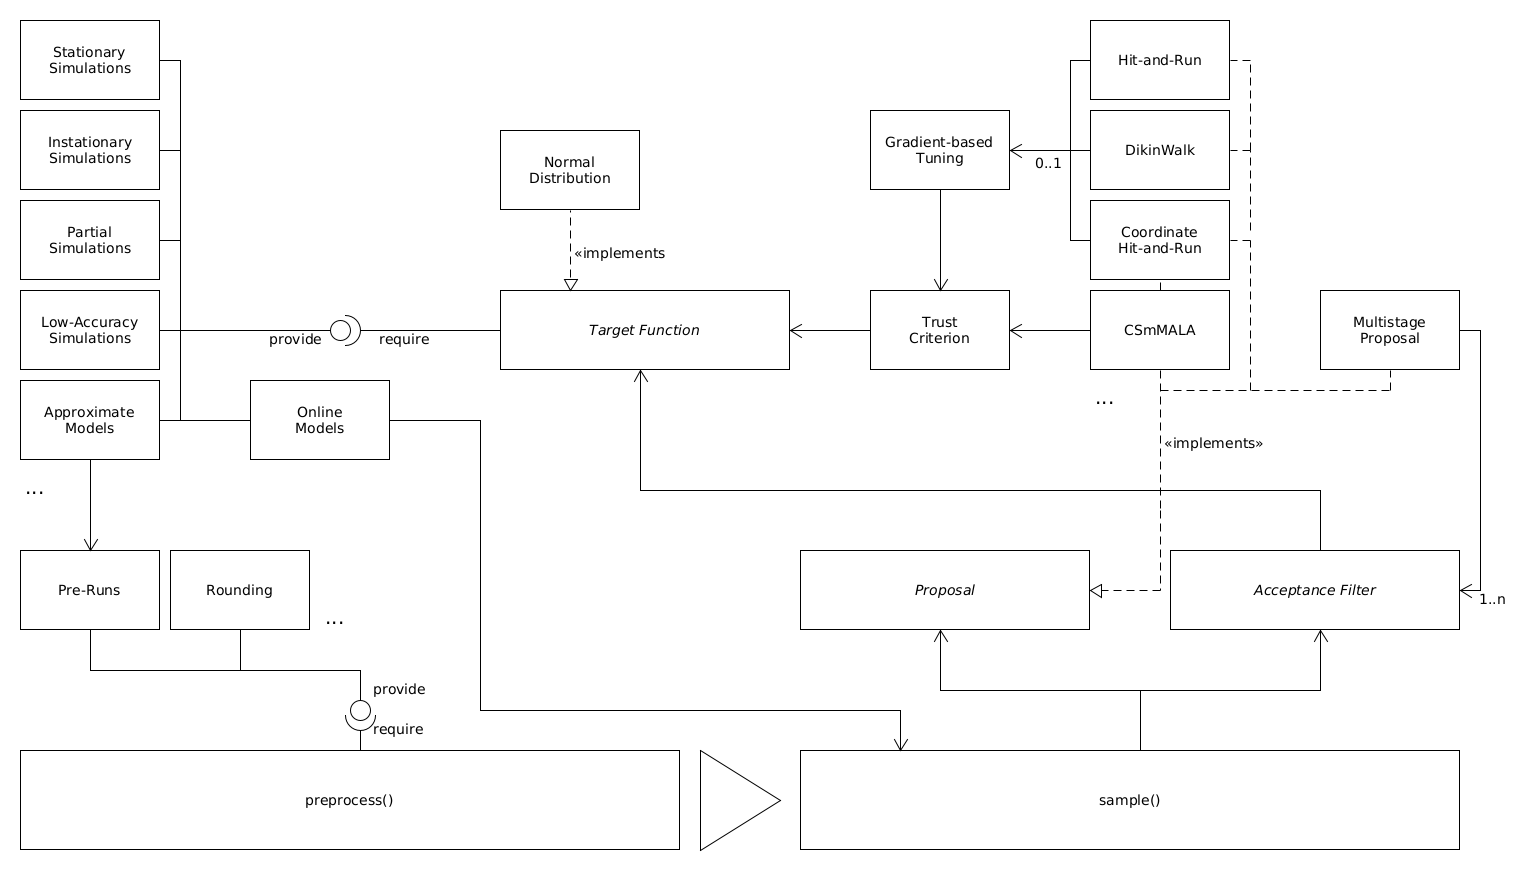
\includegraphics[width=0.7\textwidth]{hops-framework.png}
    \end{figure}
\end{frame}

\begin{frame}
    \frametitle{The framework}
    The current status
    \begin{figure}
	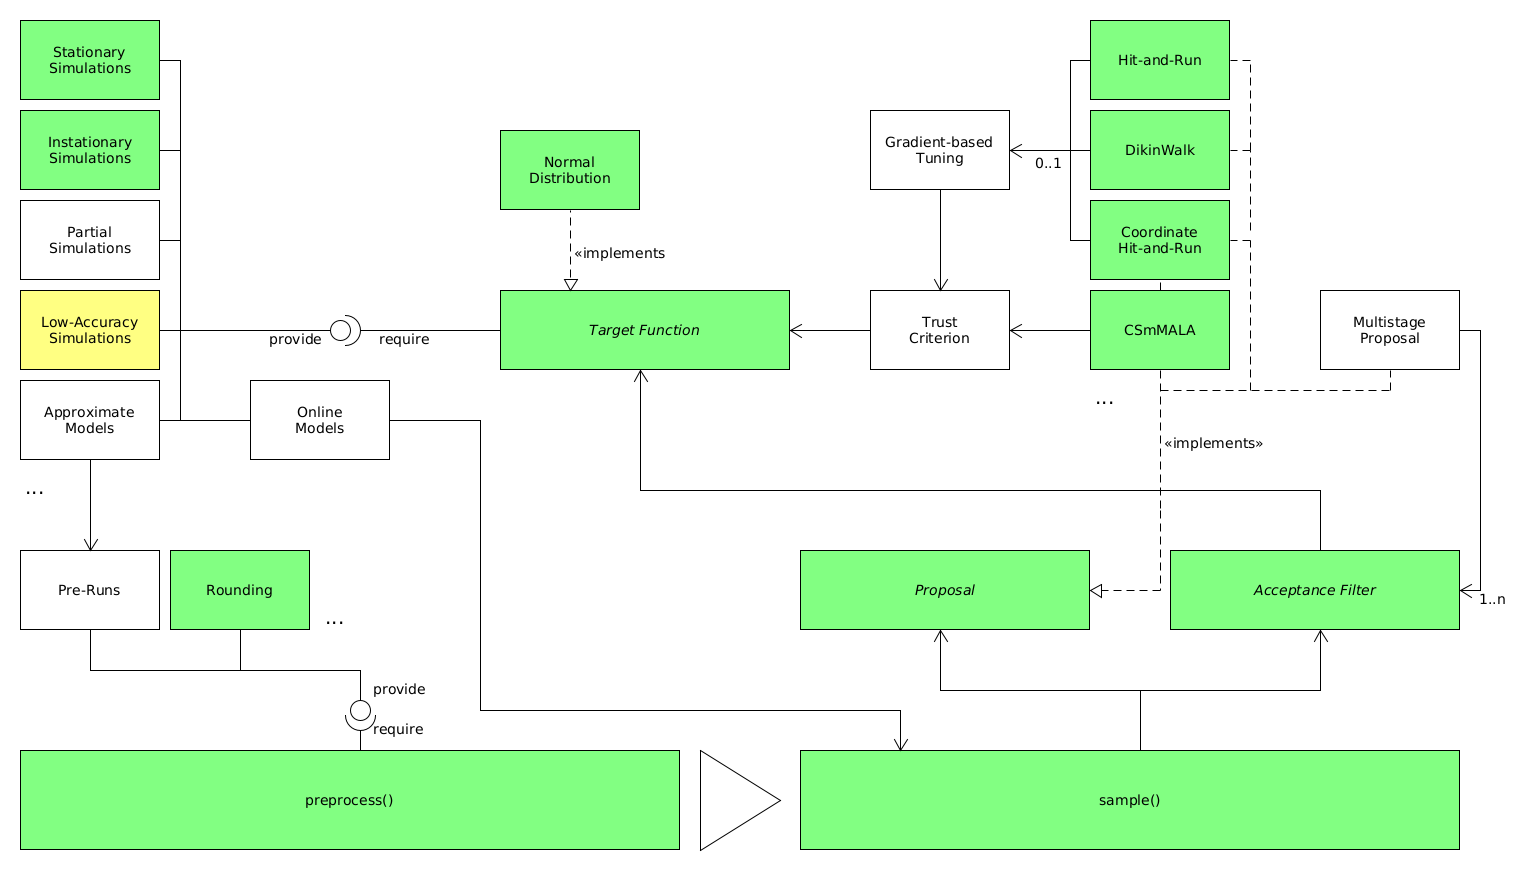
\includegraphics[width=0.7\textwidth]{hops-framework-currently.png}
    \end{figure}
\end{frame}

\begin{frame}
    \frametitle{The framework}
    Scope of this work
    \begin{figure}
	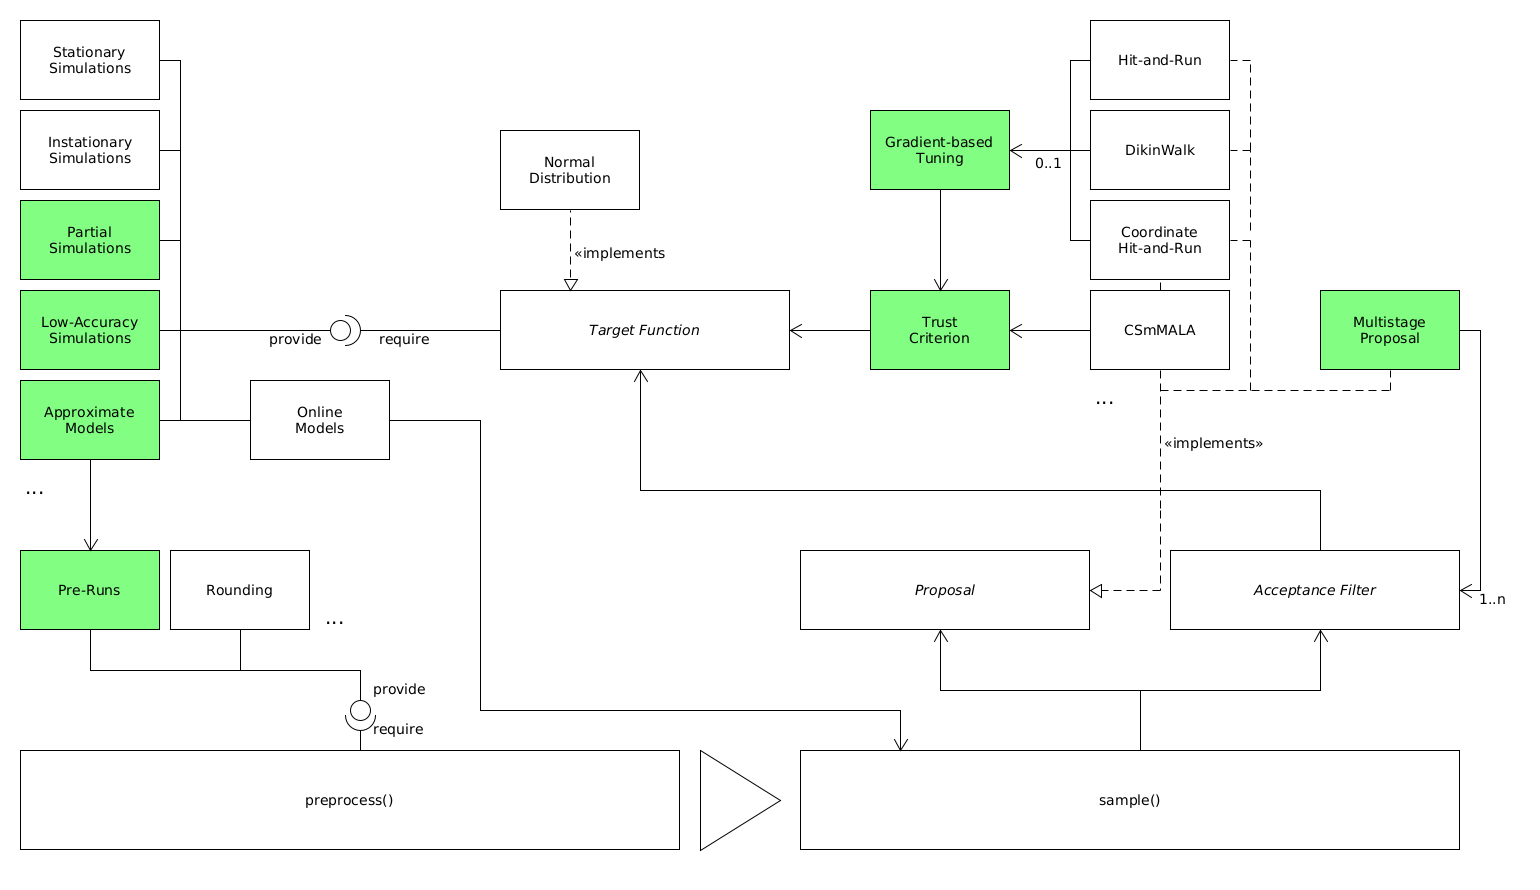
\includegraphics[width=0.7\textwidth]{hops-framework-scope.png}
    \end{figure}
\end{frame}

\begin{frame}
    \frametitle{The framework}
    Most probably beyond scope
    \begin{figure}
	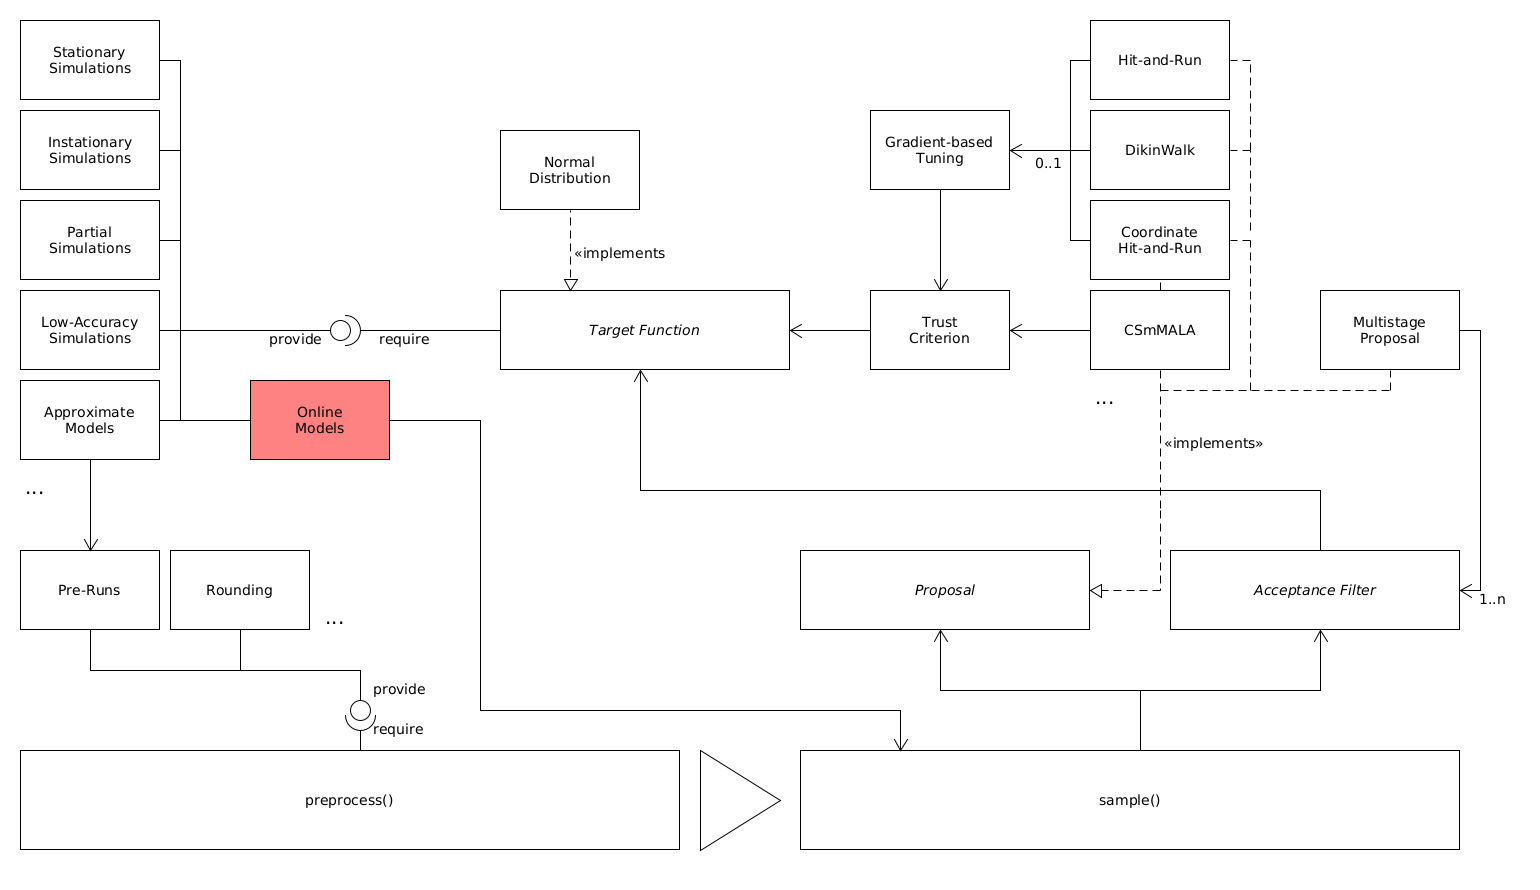
\includegraphics[width=0.7\textwidth]{hops-framework-out-of-scope.png}
    \end{figure}
\end{frame}

\begin{frame}
    \frametitle{Action Plan \& Goals} 
    \begin{itemize}
	\item Start off with proof of concept
	\begin{itemize}
	    \item Implement general framework
	    \item Use dummy simulators with artifical noise and delays 
	    \item Test approximate models and trust criterion approach with them too 
	\end{itemize}
	\item[]
	\item Develop guidelines for meaningful and effective use of the framework
	\begin{itemize}
	    \item How many stages? And what \emph{coarse} models?
	    \item Length of pre-runs? Perform pre-runs at all?
	    \item What proposal moves go well with multi-staging?
	    \item Where to use fishy models? 
	    \item Trust criterion parameters?
	    \item $\dots$
	\end{itemize}
    \end{itemize}
\end{frame}

\begin{frame}[c]{}
    \centering
    \Huge \emph{Thanks!}
\end{frame}

